Our project also includes the development of a visualisation tool for creation
and verification of several \textsc{PureCircuit} instances. We will use the
figure \ref{fig:soft:workflow} for main reference. We opted with \textit{Rust},
as the main language of development, due to its high and low level features.
From the one hand, \textit{Rust} can efficiently handle memory allocation safely
with its clever usage of the Borrower-Ownership framework. Conversely, it implements
a strongly typed system with help of generics, associated types and algebraic types
allowing us to create a versatile and compact library. Given the above, we utilise
techniques such as \texttt{Proptest}, where we create strategic randomized tests
that check whether  function follows an expected property. On the other hand
we make use of \texttt{Petgraph}, which is a sophisticated library that handles
graph-like structures in \textit{Rust}.



\begin{figure}[h!]
    \centering
    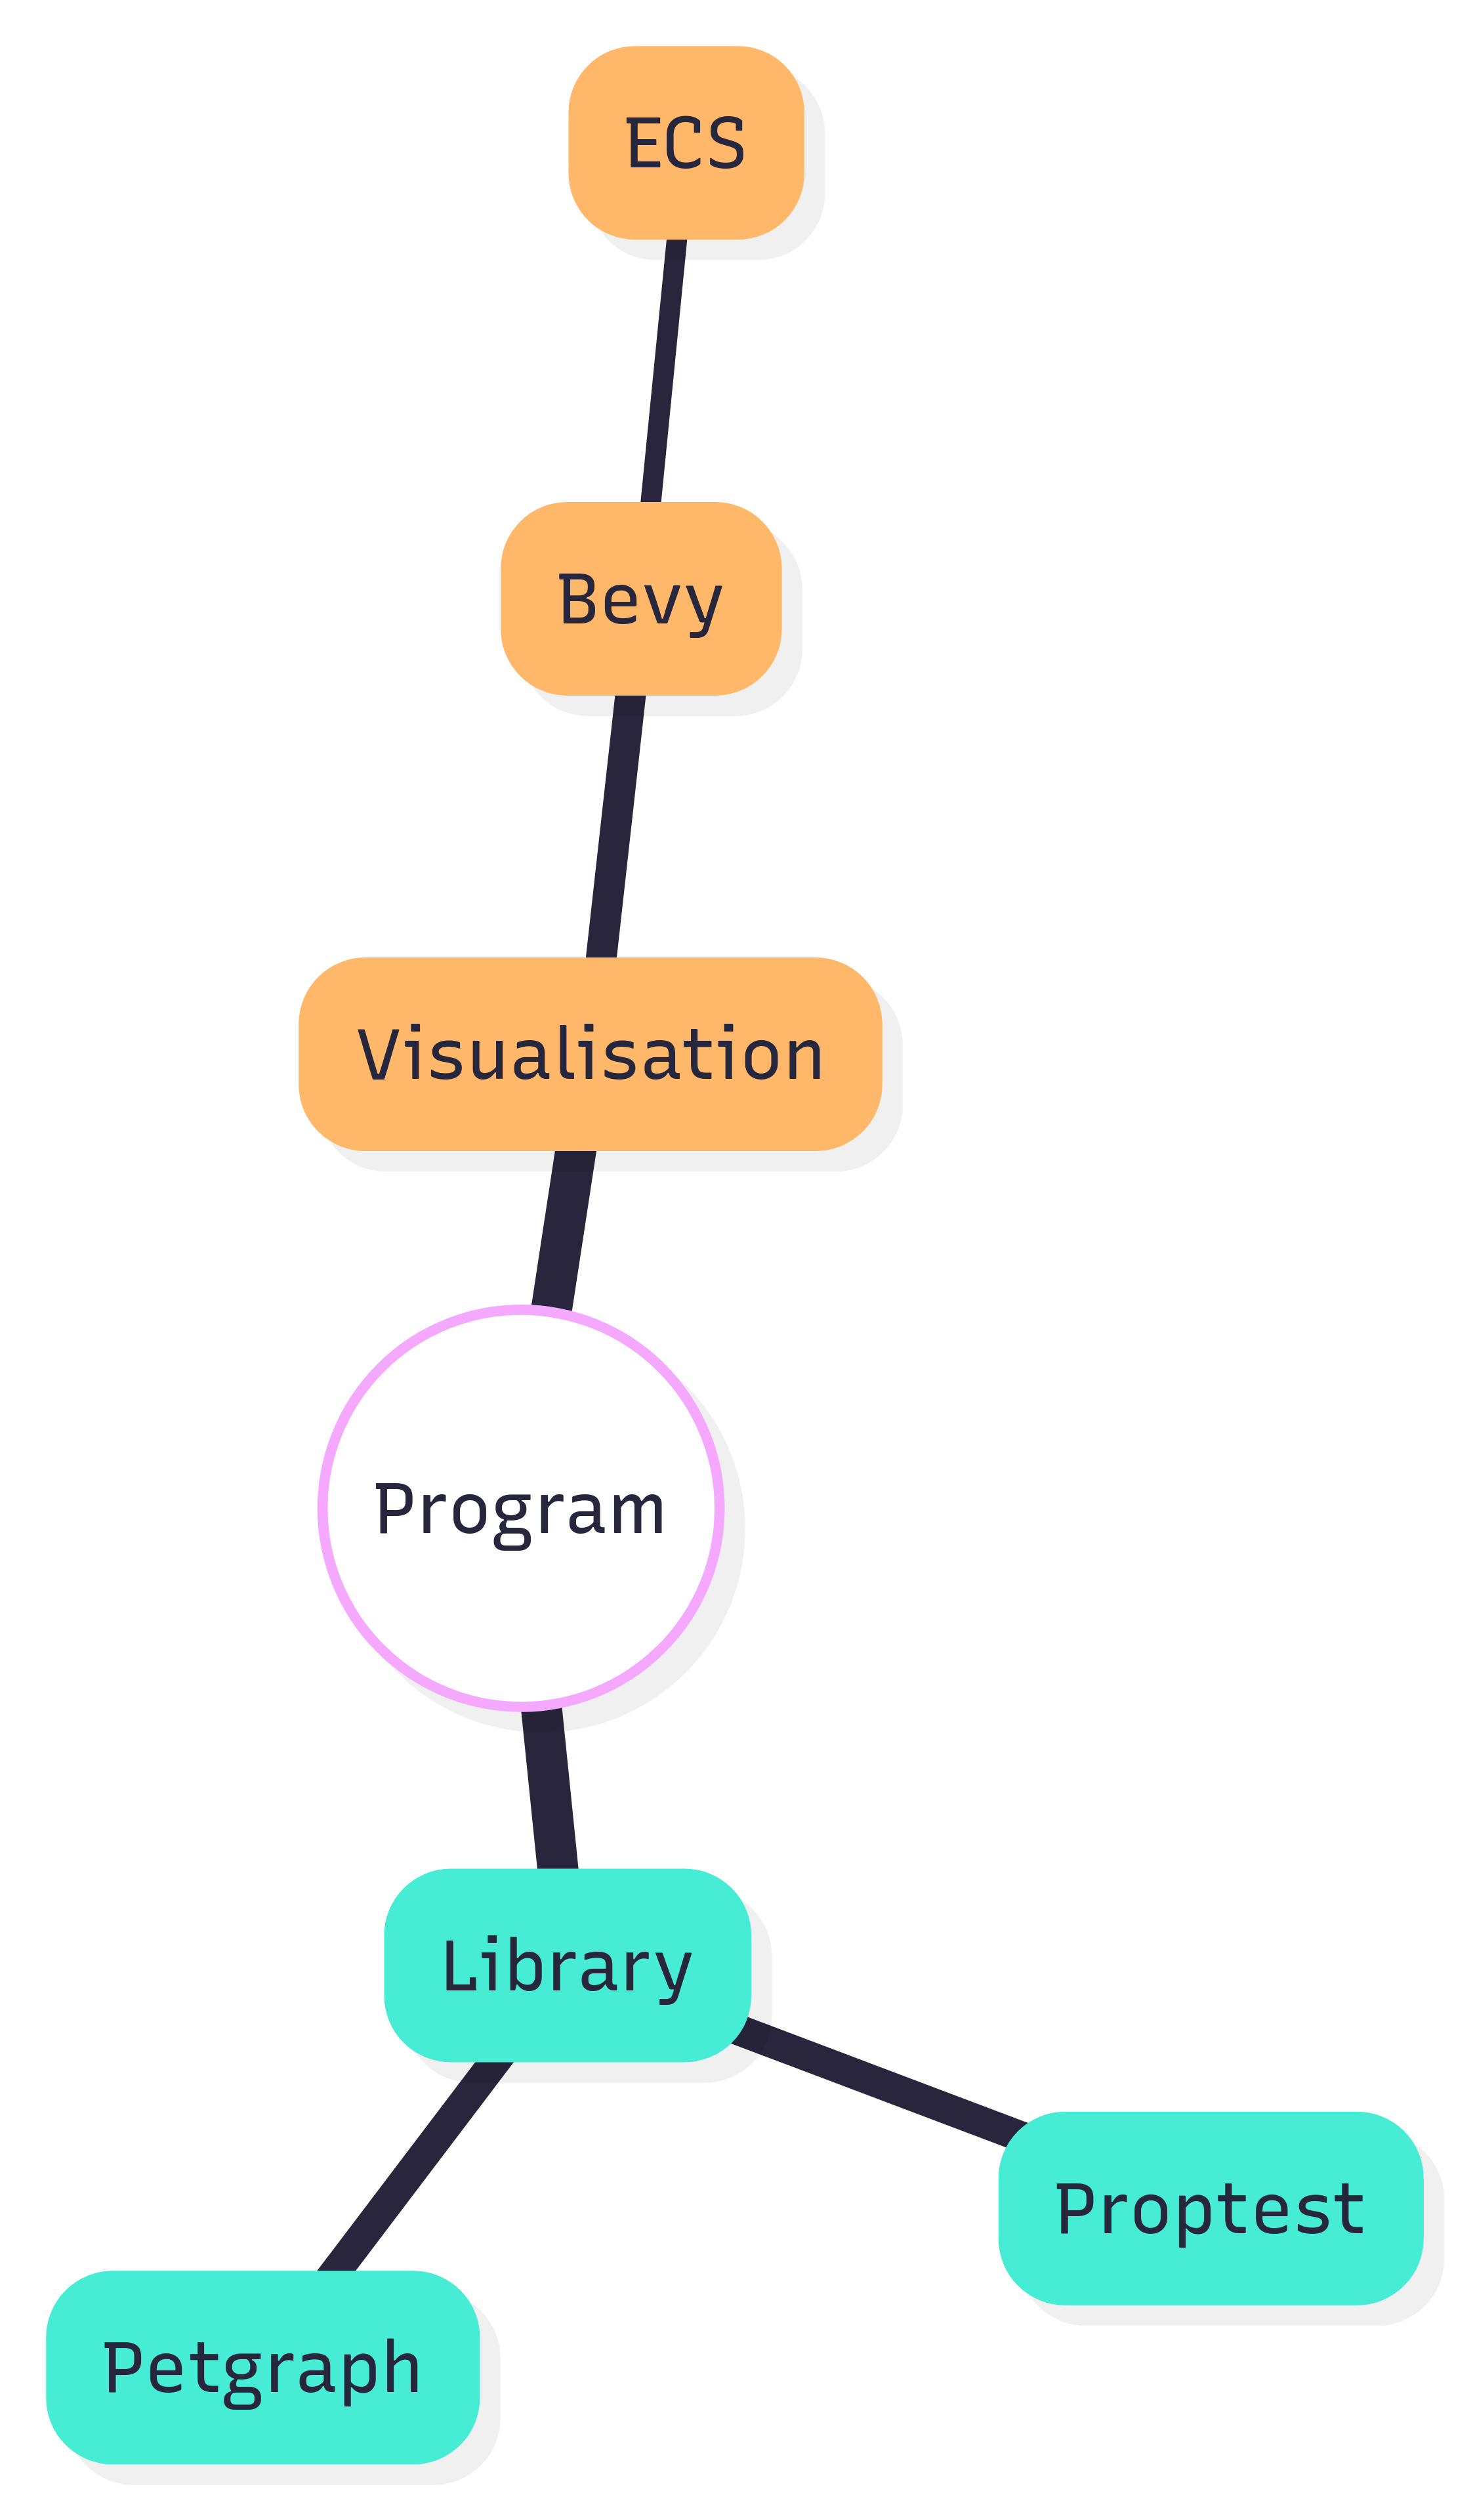
\includegraphics[width=0.35\textwidth]{assets/software-visualisation.png}
    \caption{Application workflow with respect to the libraries and dependencies use}
    \label{fig:soft:workflow}
\end{figure}


For visualisation we decided to go with \textit{Bevy}. \textit{Bevy} is a
game engine that uses the \textit{ECS} software achitecture. A general
workflow of an \textit{ECS} system can be described as such: a state 
contains entities, each of which is composed of components or properties.
A system is a specialised method that gathers entities based on their components
and describes an interaction between them. This whole process can be visualised
in the figure \ref{fig:soft:ecs-workflow}


\begin{figure}[h!]
    \centering
    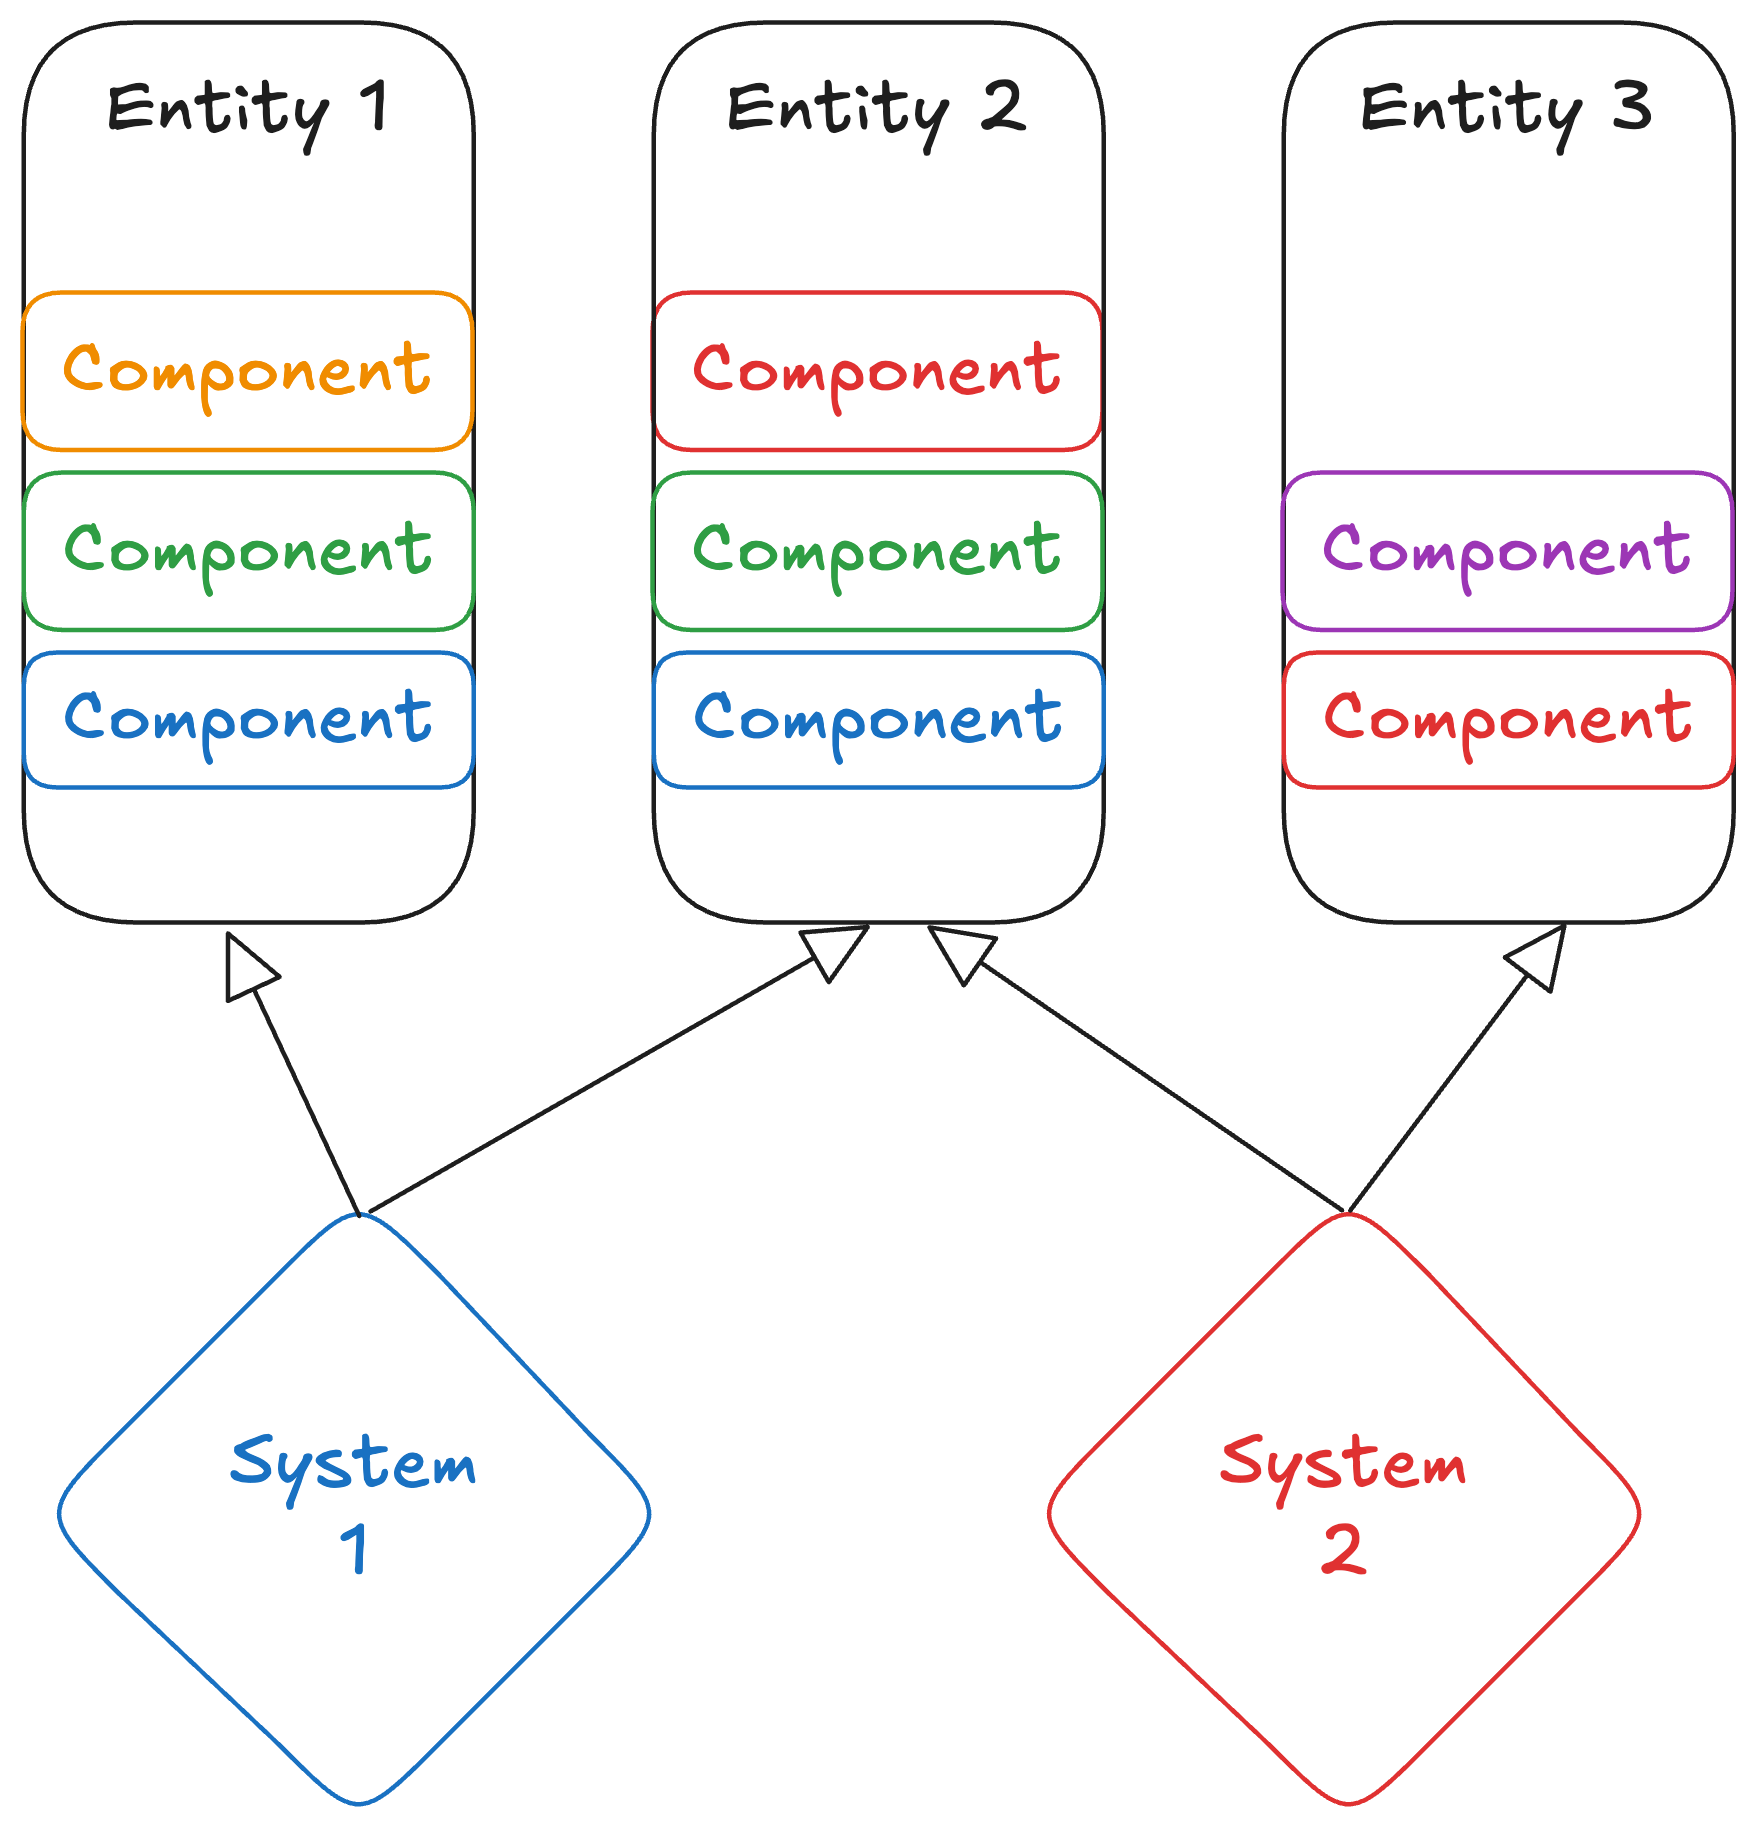
\includegraphics[width=0.35\textwidth]{assets/ECS-visualisatoin.png}
    \caption{ECS workflow visualisation}
    \label{fig:soft:ecs-workflow}
\end{figure}

\subsubsection{Current Progress}

In our introduction we referred to three main objectives. As of time of writing
we are close to the completion of the first one. We will provide a table of
objectives that have been achieved, as well as the remaining requirements needed
to complete the first milestone in \ref{tab:soft:rem-unrem-issues-stage1}. Lastly, we provide a figure
of our current visualisation in \ref{fig:soft:current-phases}

\begin{table}[h!]
    \centering
    \begin{tabularx}{0.9\textwidth}{|Y|Y|}
            \hline
            \textbf{Accomplished} & \textbf{Finished} \\
            \hhline{|==|}
            Ability to add and move nodes                                  & Add values to value nodes                                                                                   \\ \hline
            Toggle between value nodes and gate nodes                                  & Specify the type of gate to add                                                                             \\ \hline
            Add edges. Ensure that edges can only be added between heterogeneous nodes & Add indicators as to how many edges are excess/remaining for the gate to be valid                           \\ \hline  
            Move whole graph                                                           & Inclusion of a status bar as to whether the current assignment is correct, wrong or syntactically incorrect \\  \hline
            Create panel to show current state as well as some indicator and guides    &   \\ \hline
    \end{tabularx}
    \caption{Finished and remaining issues}\label{tab:soft:rem-unrem-issues-stage1}
\end{table}

%%Add image visualisation
\begin{figure}[h!]
    \centering
    \subfloat[Add nodes]{
        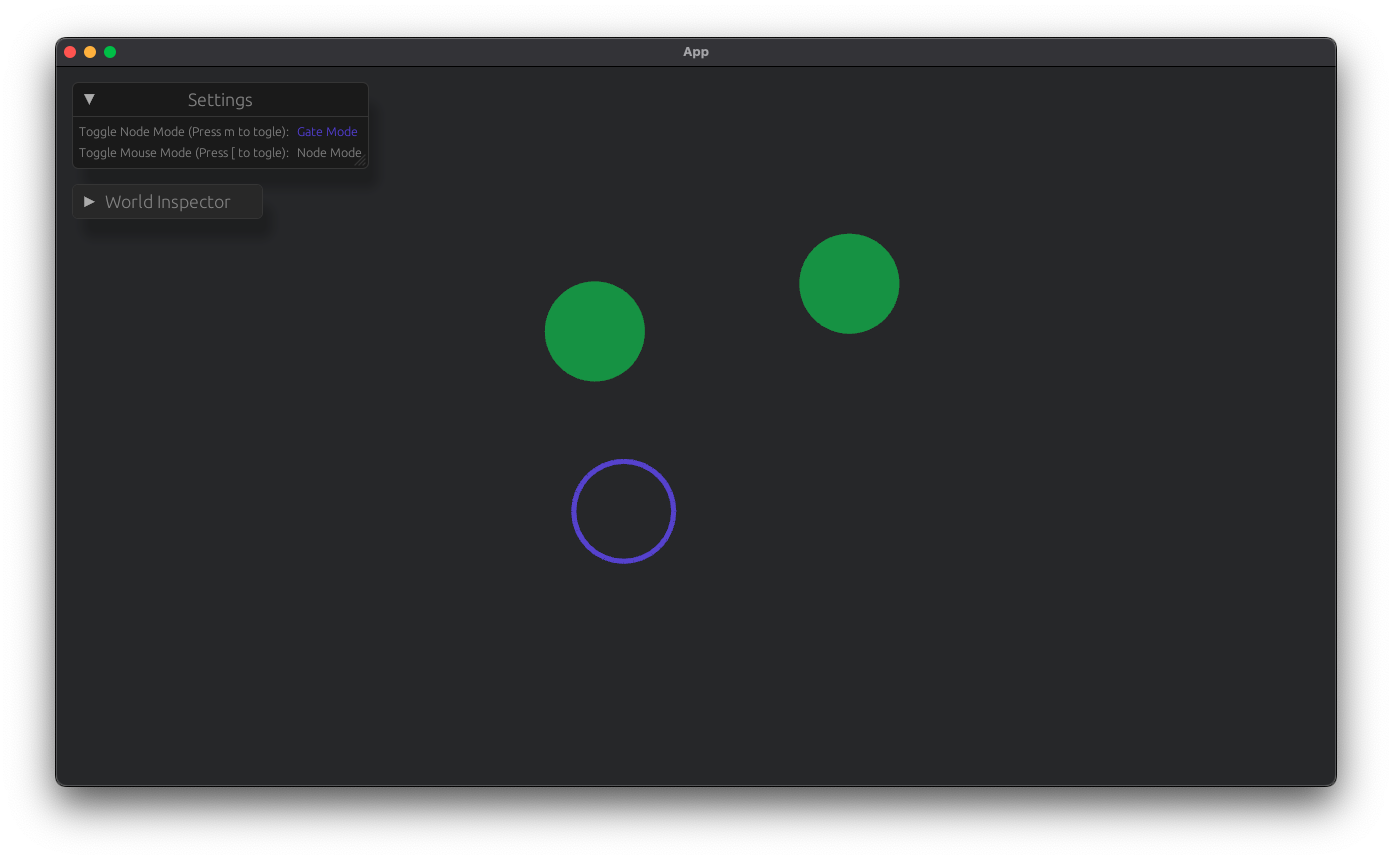
\includegraphics[width=0.3\linewidth]{assets/soft-phase-1-add-node.png}
        \label{fig:soft-phase-1:add-node}
    }
    \subfloat[Add edges]{
        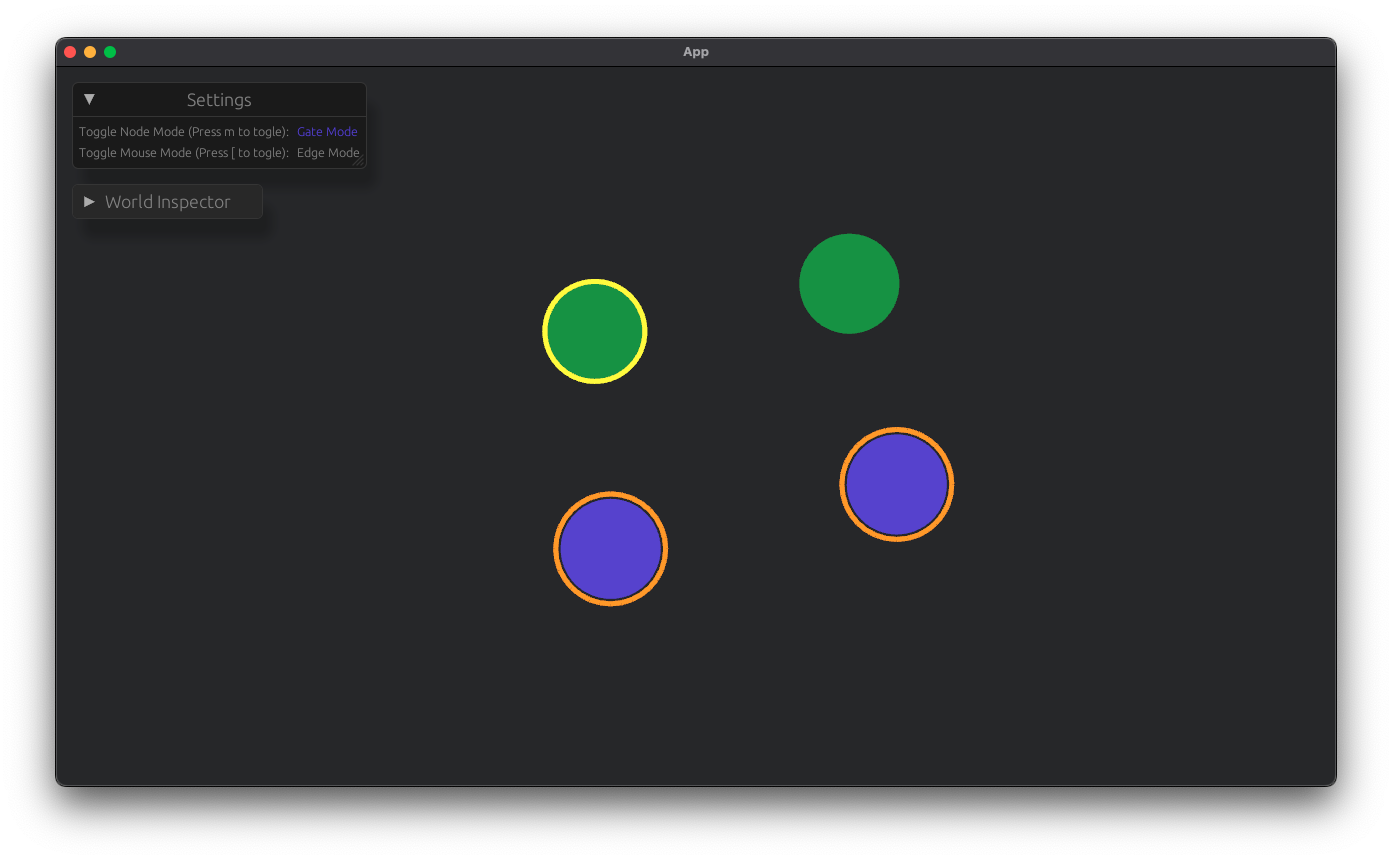
\includegraphics[width=0.3\linewidth]{assets/soft-phase-1-add-edge.png}
        \label{fig:soft-phase-1:add-edge}
    }
    \subfloat[Final state]{
        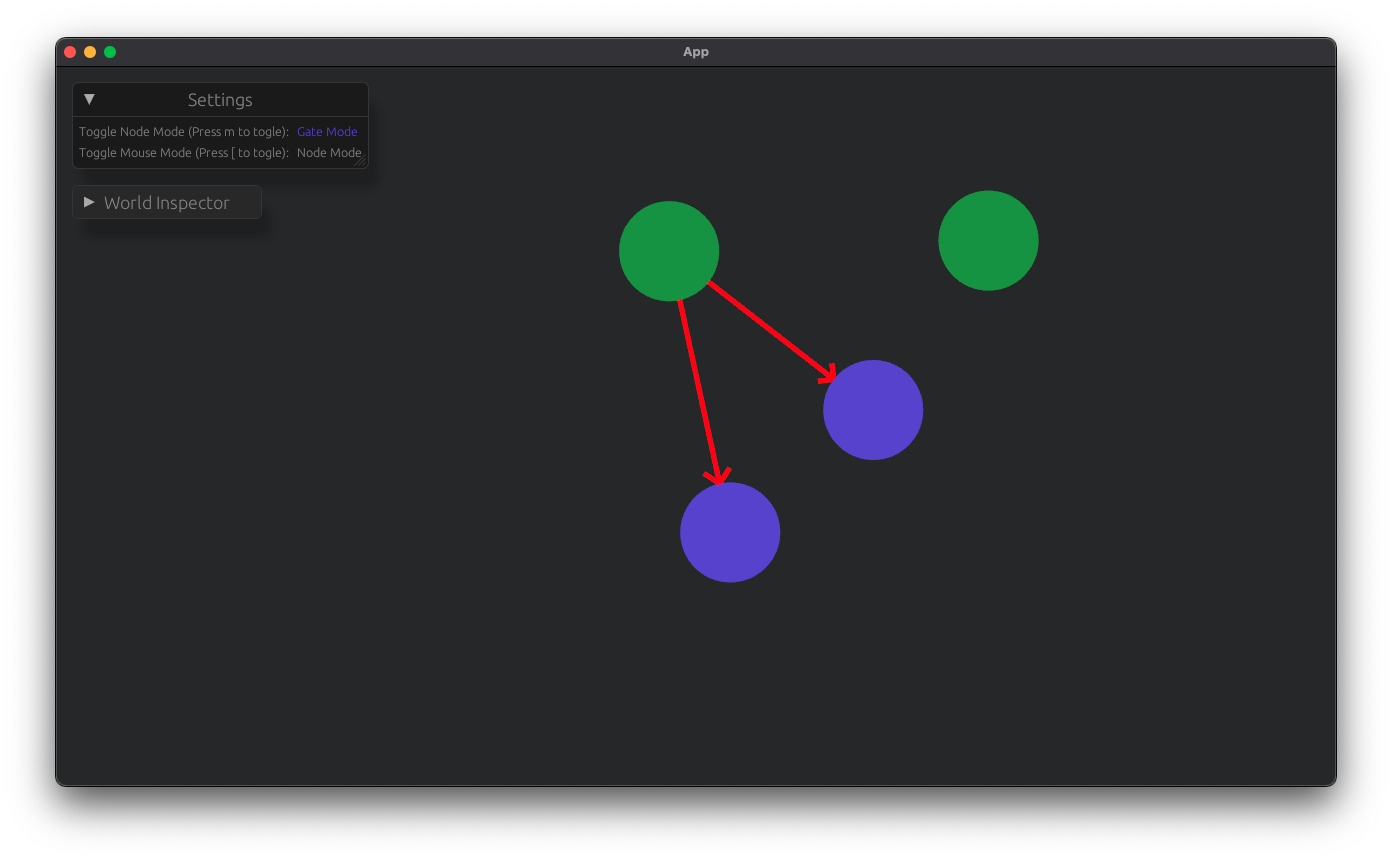
\includegraphics[width=0.3\linewidth]{assets/ soft-phase-1-final-state.png}
        \label{fig:soft-phase-1:final-state}
    }
    \caption{Screenshots of different states of the visualisation tool}
    \label{fig:soft:current-phases}
\end{figure}
\subsubsection{Next steps}

In the next steps we aim to complete the tasks that were mentioned in the above table,
as well as finding a solution or even better finding all possible solutions. Of
course due to the nature of the problem, finding a single or all solutions for big instances
is computationally difficult. We aim to investigate a method introduced by Eichelberger, where
he utilised repeated applications of the circuit to detect oscillations and replace them with
$\bot$ values. The usage of that procedure was to detect hazard but aim to utilise that procedure
as a heuresaaaawtical approach to reach a satisfying assignment. We do not primarily aim
to fully optimise these algorithms, as the project focuses more on analysing the theoritical findings
of \textsc{PureCircuit}.





